\chapter{\heiti \label{ch3} 非配对图片的图像迁移算法}

\section{\heiti \label{sec:2.1}算法流程}
\begin{algorithm}[thb]
	\caption{k, is a hyperparameter.We used k = 1, the least expensive option, in our experiments}
    \label{alg}
	\begin{algorithmic}[1]
	\REQUIRE  图片A数据集 $\mathbf{R}$,  图片B数据集 $\mathbf{X}$,迭代次数 n 
    \FOR{$i = 1$ to $n$}
      \STATE\FOR{$i = 1$ to $k$}
      \STATE Sample minibatch of m noise Samples from noise prior Pg(z)
      \STATE Sample minibatch of n examples from data generationg districution Pdata(x)
      \STATE Update the discriminator by ascending its stochastic gradient:
      \STATE \begin{align}
        \bigtriangledown_{\theta_{d}} 1/M \sum_{n=1}^M [\log D(x^{i}) + \log (1-D(G(z^{i})))]
      \end{align}
      \STATE\ENDFOR
      \STATE Sample minibatch of m noise Samples from noise prior Pg(z)
      \STATE Update the discriminator by decending its stochastic gradient:
      \STATE \begin{align}
        \bigtriangledown_{\theta_{g}} 1/M \sum_{n=1}^M \log (1-D(G(z^{i})))
      \end{align}
    \ENDFOR

	\end{algorithmic}
\end{algorithm}

\section{\heiti \label{sec:2.2}实验数据集}

\subsection{\heiti 数据集来源}
本次实验数据集来源为原作者提供的数据集,数据集来源:\url{https://people.eecs.berkeley.edu/~taesung_park/CycleGAN/datasets/}

\section{\heiti \label{sec:2.2}实验结果}
The experimental results are shown in the figure\ref{fig:change}\ref{fig:change2}\ref{fig:loss_200_20}.

\begin{figure}[thb]
\centering
\subfigure{
  \label{subfig:contour-Lastfm-VDCMF-PAKDD}
  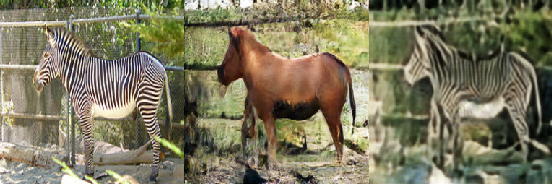
\includegraphics[width=0.65\textwidth]{images/Test_result_86.png}}
  \space \space \space \space \space \space \space
 \subfigure{
  \label{subfig:contour-Epinions-VDCMF-PAKDD}
  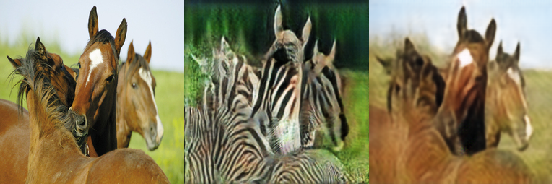
\includegraphics[width=0.67\textwidth]{images/Test_result_2.png}}
\caption{}
\label{fig:change2}
\centering
    \subfigure{
      \label{subfig:contour-Lastfm-VDCMF-PAKDD}
      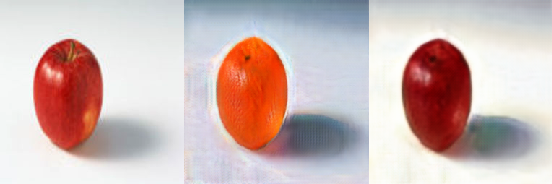
\includegraphics[width=0.65\textwidth]{images/Test_result_164.png}}
      \space \space \space \space \space \space \space
     \subfigure{
      \label{subfig:contour-Epinions-VDCMF-PAKDD}
      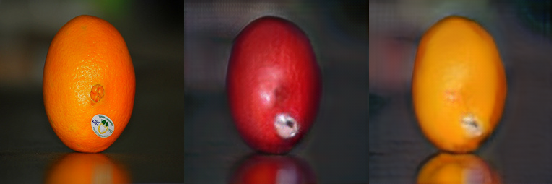
\includegraphics[width=0.67\textwidth]{images/Test_result_235.png}}
  \caption{Basically, the conversion between unpaired images and images has been implemented, but the conversion effect is not very good, and the converted image is not smooth enough. In the pixel processing, our model still needs improvement.}
  \label{fig:change}

      \includegraphics[width=0.67\textwidth]{images/loss200_02.pdf}
  \caption{As the epoch continues to increase,
  the accuracy of GA and GB 
  keep rising and gradually stabilizes.
  the stable values of $D_A$ is about 0.83,
  the stable values of $D_B$ is about 0.76.}
  \label{fig:loss200_02}
\end{figure}



\section{\heiti 不同图像迁移算法性能比较}

As shown in the table\ref{table:performance}, 
Cyclegan basically realizes the conversion 
between unpaired pictures, 
but the image conversion effect is slightly 
worse than other image migration algorithms. 
The results obtained from the experiment do 
not affect the intuitive judgment of the human eye.

\begin{table}[htb]
  \center
  \caption{}
  \label{table:performance}
  \resizebox{1\textwidth}{!}{
  \begin{tabular}{|c|c|c|c|c|c|c|c|c|}
  \hline
   &\multicolumn{1}{|c|}{Map to Photo}& \multicolumn{1}{|c|}{Photo to  Map}\\
  \hline
   & Error rate  &  Error rate\\
  \hline
  CoGAN\cite{CoGAN} & 1.1\% & 1.4\% \\
  SimGAN\cite{SimGAN} &1.6\% & 2.8\% \\
  CycleGAN(our) & 23.6\% &22.4\% \\
  
  \hline
  \end{tabular}
  }
  \end{table}


\section{\heiti 算法参数的影响}
When obtaining the optimal parameters of the model,
 we use the small epoch to continuously test the optimal parameters of the approximation model. 
 Finally, the learning rate is best around 0.002.

\begin{figure}[htbt]
  \centering
    \subfigure{
      \label{subfig:loss200_02}
      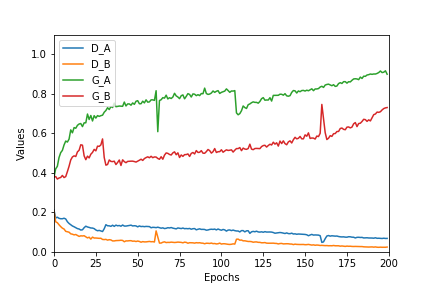
\includegraphics[width=6cm,height = 5cm]{images/loss_200_02.png}}
      \space \space \space \space \space \space \space
     \subfigure{
      \label{subfig:loss20_02}
      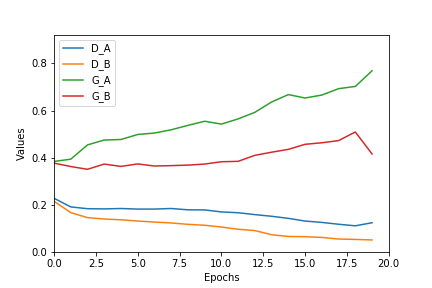
\includegraphics[width=6cm ,height=5cm]{images/loss_20_02.png}}
  \caption{The epoch value increases and 
  the value increases when the 
  accuracy reaches stability.}
  \label{fig:loss_200_20}
  
  \centering
    
     \subfigure{
      \label{subfig:loss20_015}
      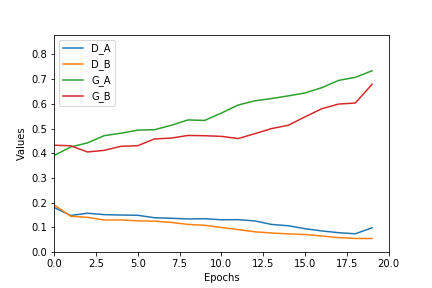
\includegraphics[width=0.67\textwidth]{images/loss_20_015.png}}
      \subfigure{
      \label{subfig:loss20_030}
      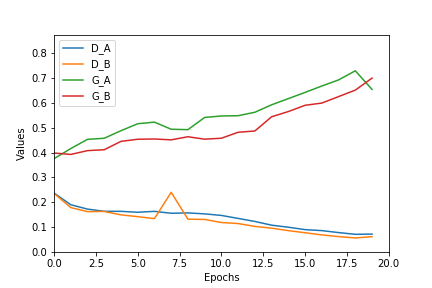
\includegraphics[width=0.67\textwidth]{images/loss_20_030.png}}
  \caption{When the learning rate is equal to 0.003, there is an over-fitting phenomenon. When the learning rate is 0.0015, the image is slightly worse than the learning rate of 0.002.}
  \label{fig:loss_02_015_030}
  
\end{figure}








